\documentclass[platex]{jsarticle}  
\usepackage{cslreport}
\usepackage{amsmath}
\usepackage{amsthm}
\usepackage[hang,small,bf]{caption}
\usepackage[subrefformat=parens]{subcaption}
\captionsetup{compatibility=false}
\usepackage[dvipdfmx]{graphicx}
\usepackage[dvipdfmx]{xcolor}
\usepackage{here}

\title{セミナー用テンプレート}
\author{動的システム・ロボティクス研究室 \quad B4 \quad 田辺 裕翔}
\date{2025年 10月 21日}
\repnum{dsr25re01}

\begin{document}
\maketitle
\section{はじめに}
先月は状態推定についてのまとめを行った。今回は、まとめ直したことによって出てきた問題点の改善を行った。次に今後の方針についての考えを軽く話す。

\section{状態推定}
前回の状態推定の結果をFig.\ref{fig:old002g}$\sim$\ref{fig:old002ip}に示す。紫の実線がUVA/Pdovaの応答、青の実践がssogmmの応答、赤のドットがEKFの推定結果、黄色のドットがオブザーバによる推定結果を表している。拡張カルマンフィルタによる推定結果に対してオブザーバの推定結果は状態Xについてのみ誤推定が発生している。
この問題点についてはオブザーバゲインが思っていたよりもバランスが悪くなっていただけなので、そこを修正した。
またもう一つ問題点が見つかった。拡張カルマンフィルタのコードにミスがあった。転置しなければならない行列を一つ転置していなかった。
コードを修正してシミュレーションをすると、オブザーバと同じように状態Xについてのみ誤推定が出た。そのため拡張カルマンフィルタについても重みの調整を行った。
これ以上は細かい調整になりそうだというとこで、調整を終えて、シミュレーションをした結果がFig.\ref{fig:002g}$\sim$\ref{fig:002ip}に示す通りである。
青の実線がUVA/Padovaの応答、紫の実線がssogmmの応答、赤のドットがオブザーバの推定結果、黄色のドットがEKFによる推定結果を表している。
全ての状態がうまく収束していることがわかる。またオブザーバに対して拡張カルマンフィルタの方が収束が早いことがわかる。
シミュレーション全体(4日間)でのRMSEと4日目のみのRMSEをTable.\ref{tb:rmse}に示す。RMSEはUVA/Padova T1DMシミュレータから得られた血糖値に対する状態推定誤差である。
このTable.\ref{tb:rmse}からも拡張カルマンフィルタによる状態推定結果の方がオブザーバよりも精度が良いことがわかる。
今後のmpcの実装を考えても状態の収束は早い方が都合が良いため、状態推定器としては拡張カルマンフィルタの方がいい。
\begin{table}[htbp]
  \centering
    \caption{RMSE}
   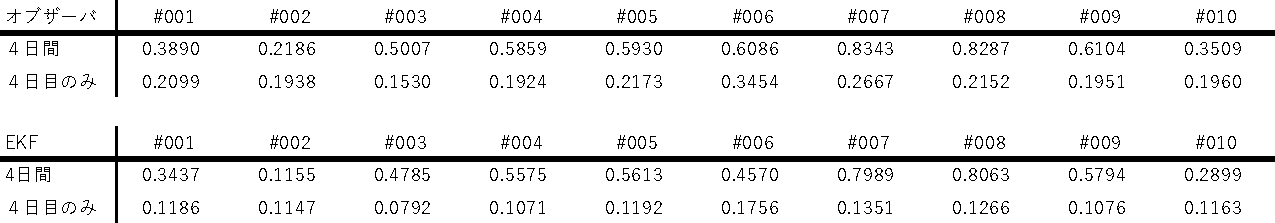
\includegraphics[width=\columnwidth]{fig/rmse.pdf}
  \label{tb:rmse}
\end{table}

\begin{figure}[H]
  \centering
  \begin{minipage}{0.65\columnwidth}
     \centering
     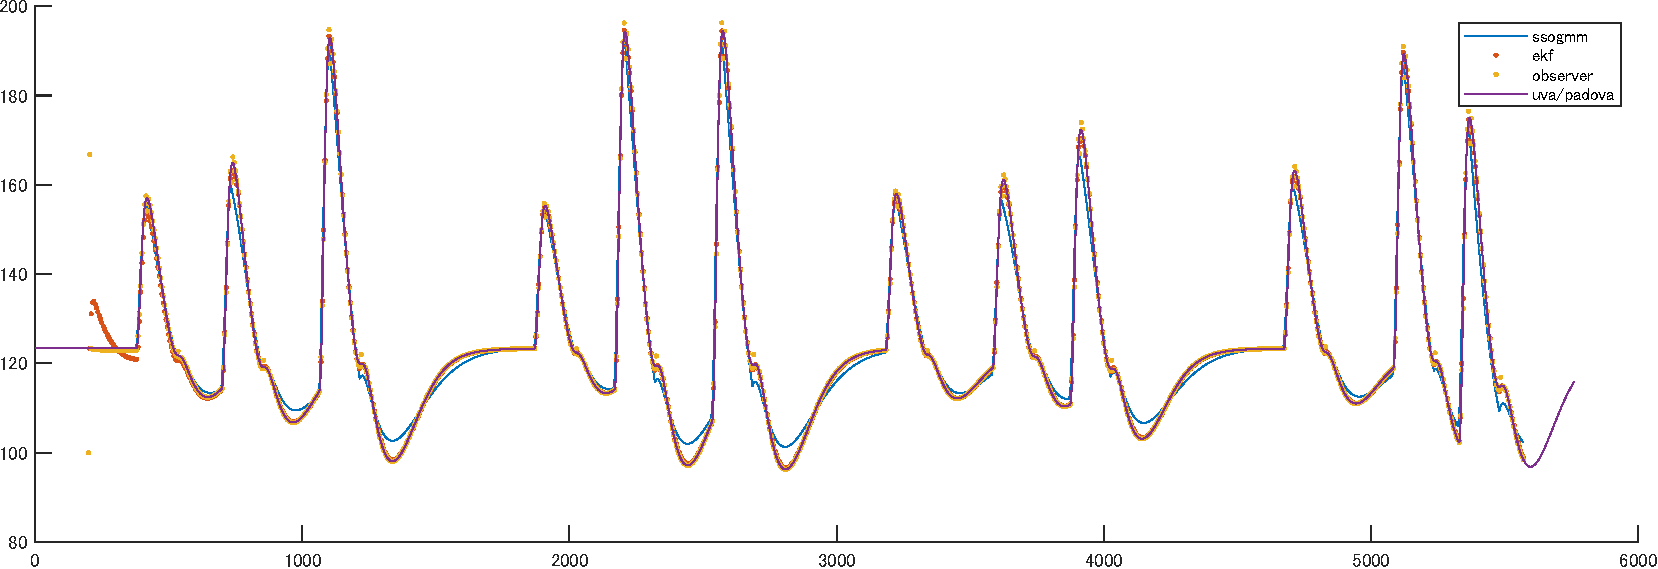
\includegraphics[width=\columnwidth]{fig/old002g.pdf}
     \caption{G}
     \label{fig:old002g}
  \end{minipage}
%
  \begin{minipage}{0.65\columnwidth}
     \centering
     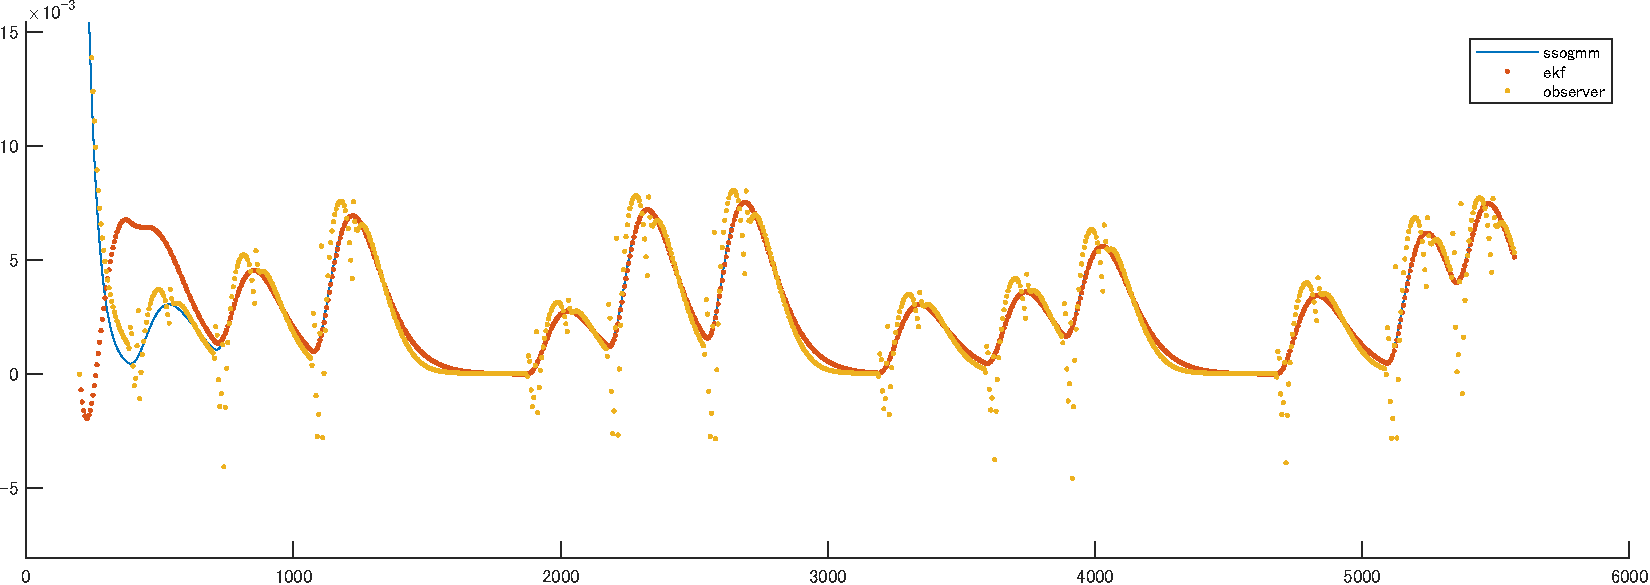
\includegraphics[width=\columnwidth]{fig/old002x.pdf}
     \caption{X}
     \label{fig:old002x}
  \end{minipage}
%
  \begin{minipage}{0.65\columnwidth}
     \centering
     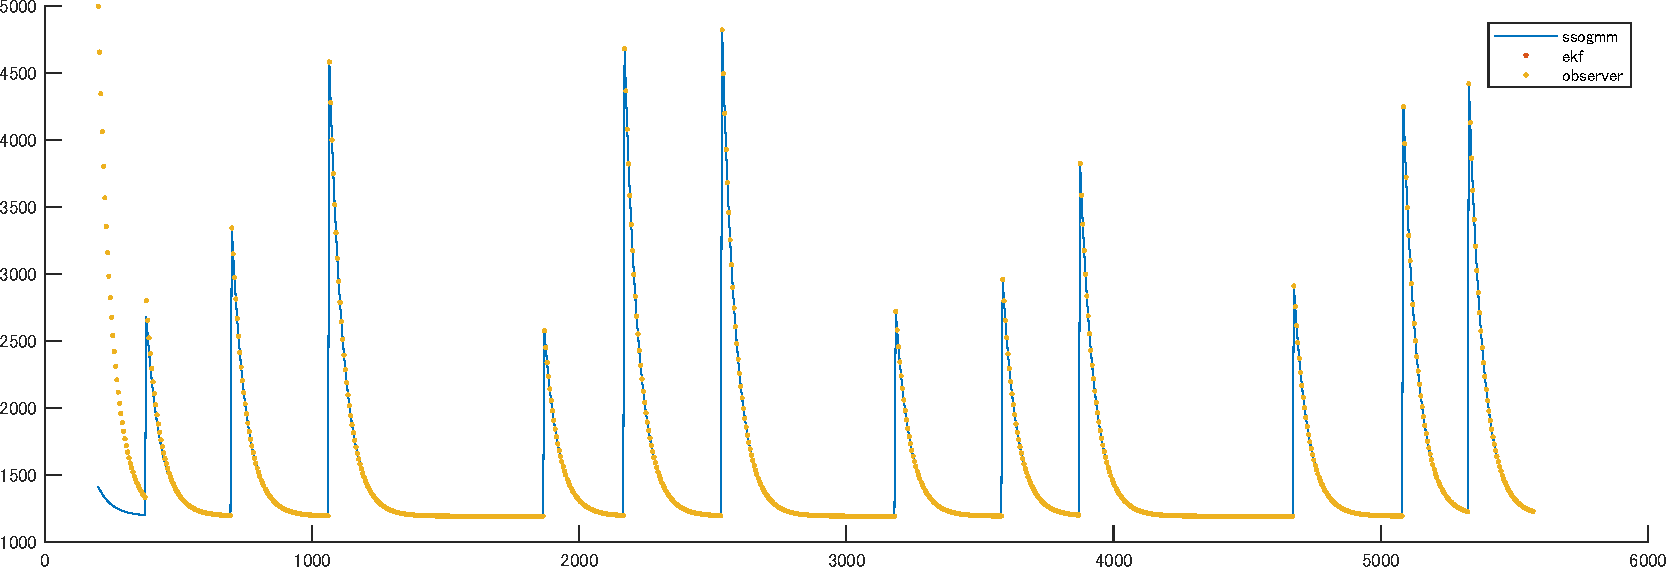
\includegraphics[width=\columnwidth]{fig/old002i1.pdf}
     \caption{I1}
     \label{fig:old002i1}
  \end{minipage}
%
  \begin{minipage}{0.65\columnwidth}
     \centering
     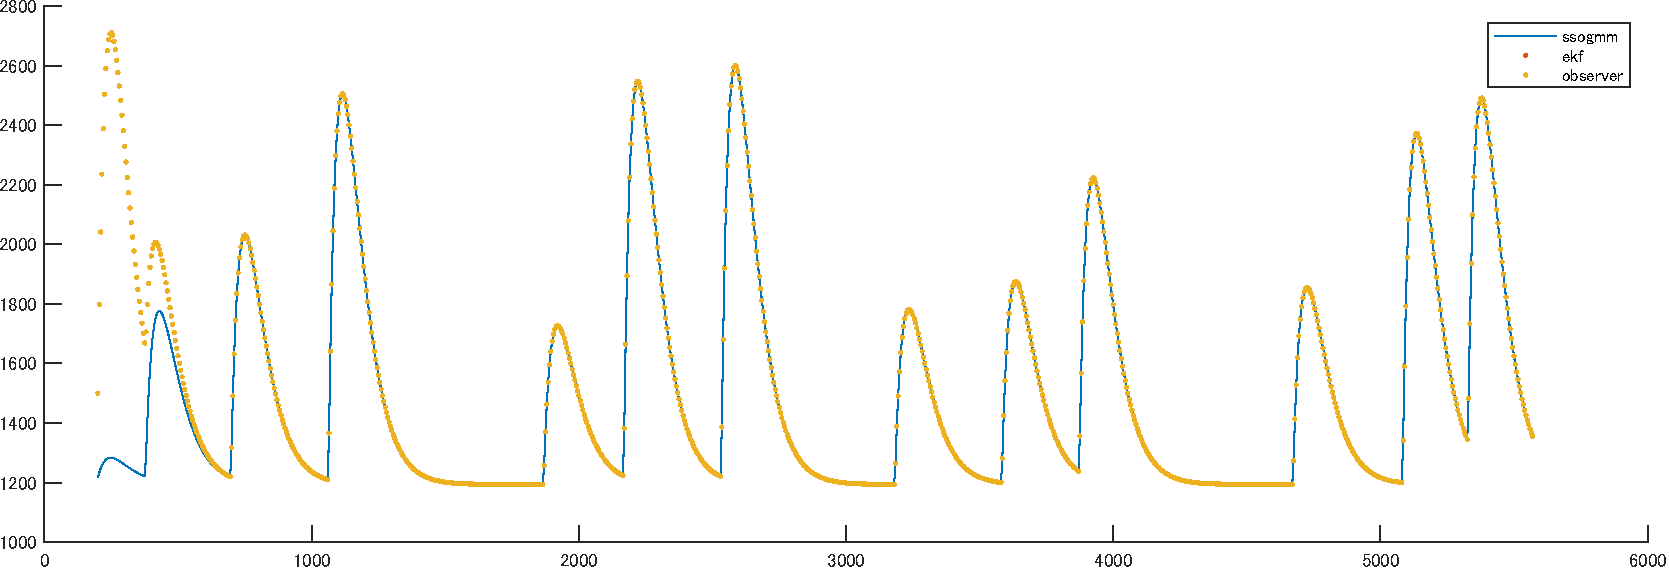
\includegraphics[width=\columnwidth]{fig/old002i2.pdf}
     \caption{I2}
     \label{fig:old002i2}
  \end{minipage}
%
  \begin{minipage}{0.65\columnwidth}
     \centering
     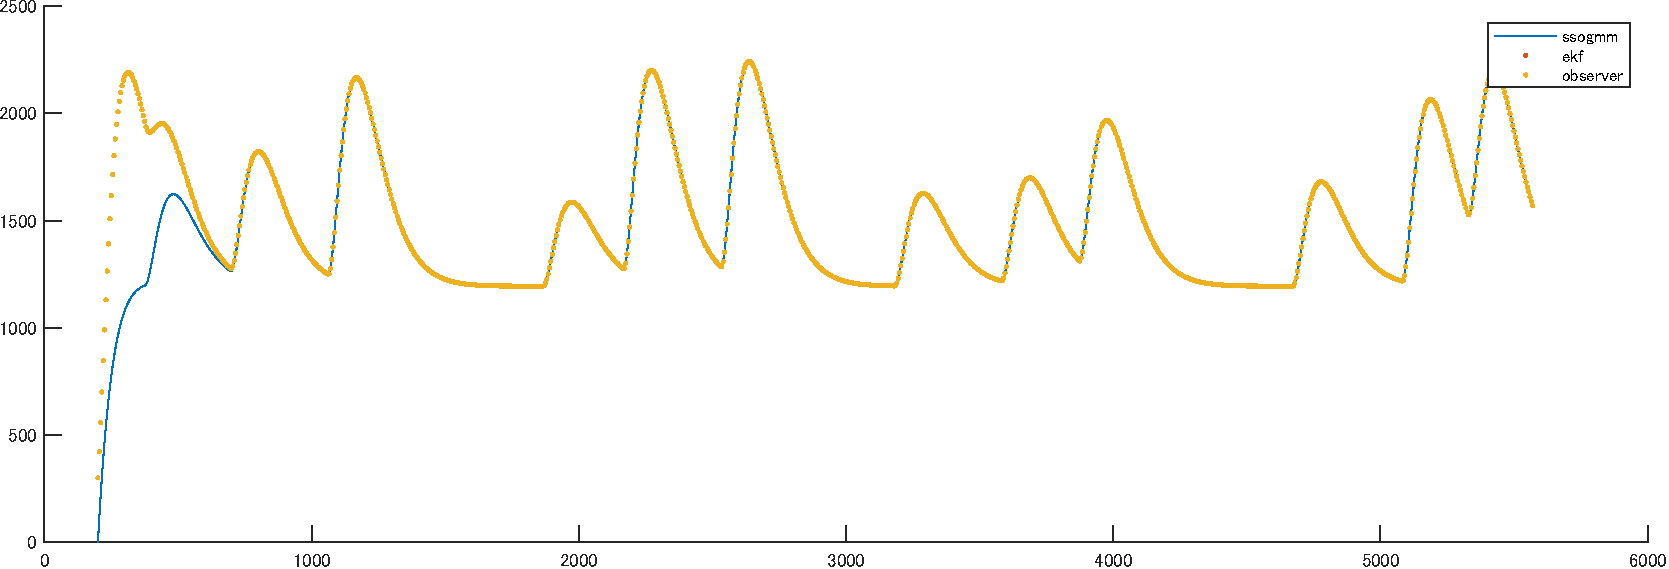
\includegraphics[width=\columnwidth]{fig/old002ip.pdf}
     \caption{Ip}
     \label{fig:old002ip}
  \end{minipage}
\end{figure}



\begin{figure}[H]
  \centering
  \begin{minipage}{0.65\columnwidth}
     \centering
     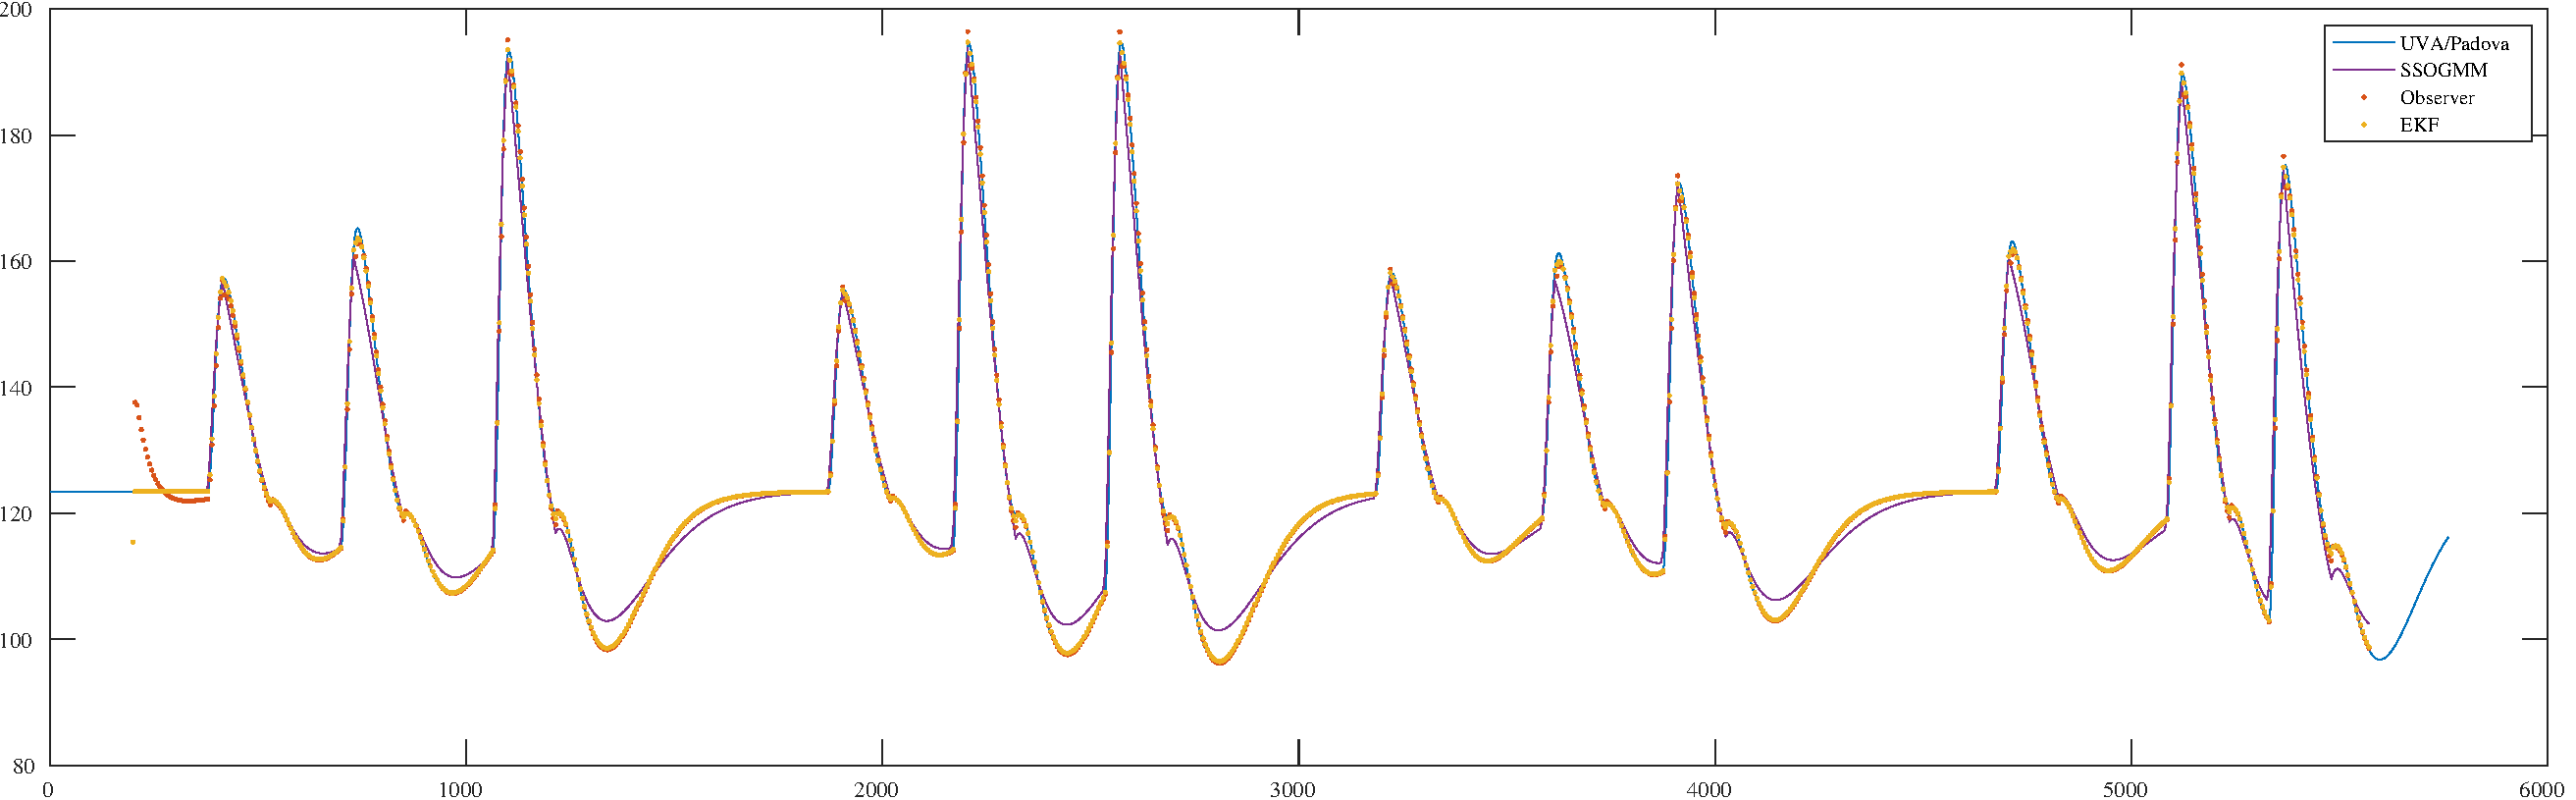
\includegraphics[width=\columnwidth]{fig/002g.pdf}
     \caption{G}
     \label{fig:002g}
  \end{minipage}
%
  \begin{minipage}{0.65\columnwidth}
     \centering
     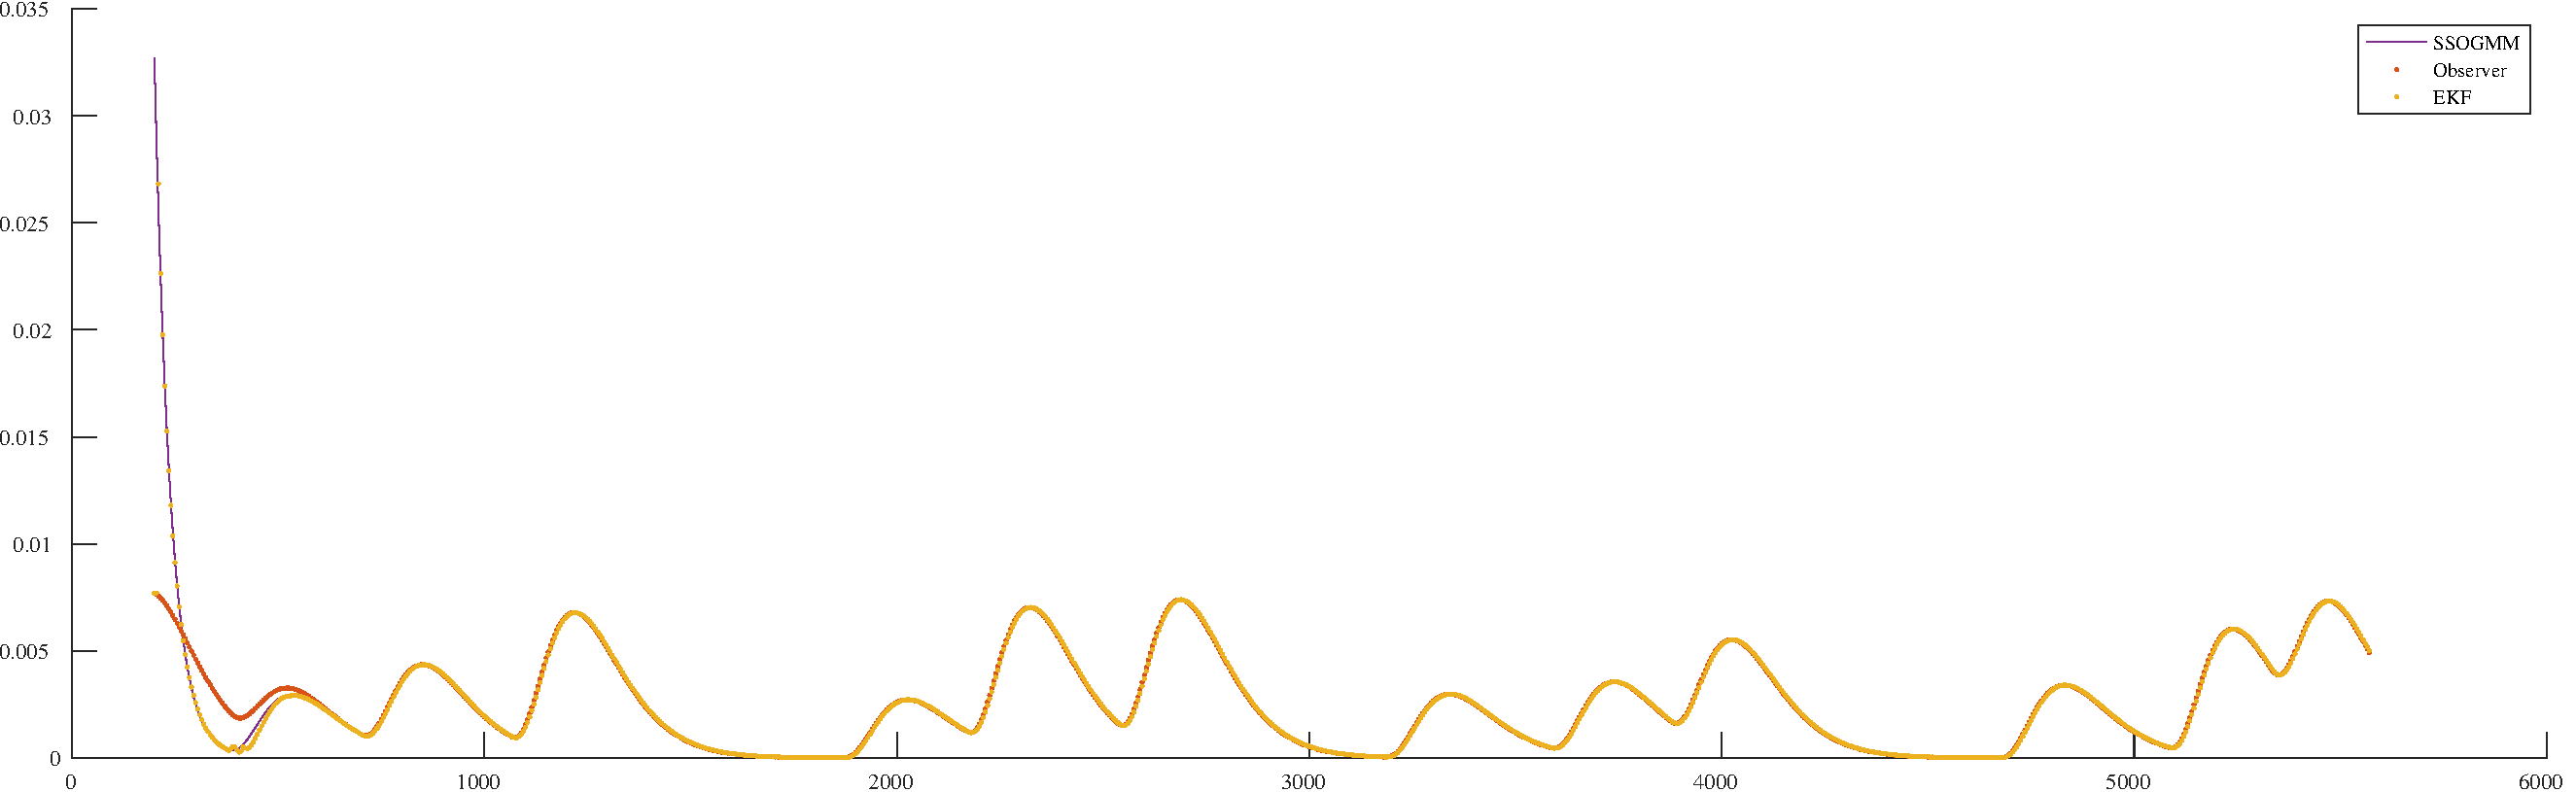
\includegraphics[width=\columnwidth]{fig/002x.pdf}
     \caption{X}
     \label{fig:002x}
  \end{minipage}
%
  \begin{minipage}{0.65\columnwidth}
     \centering
     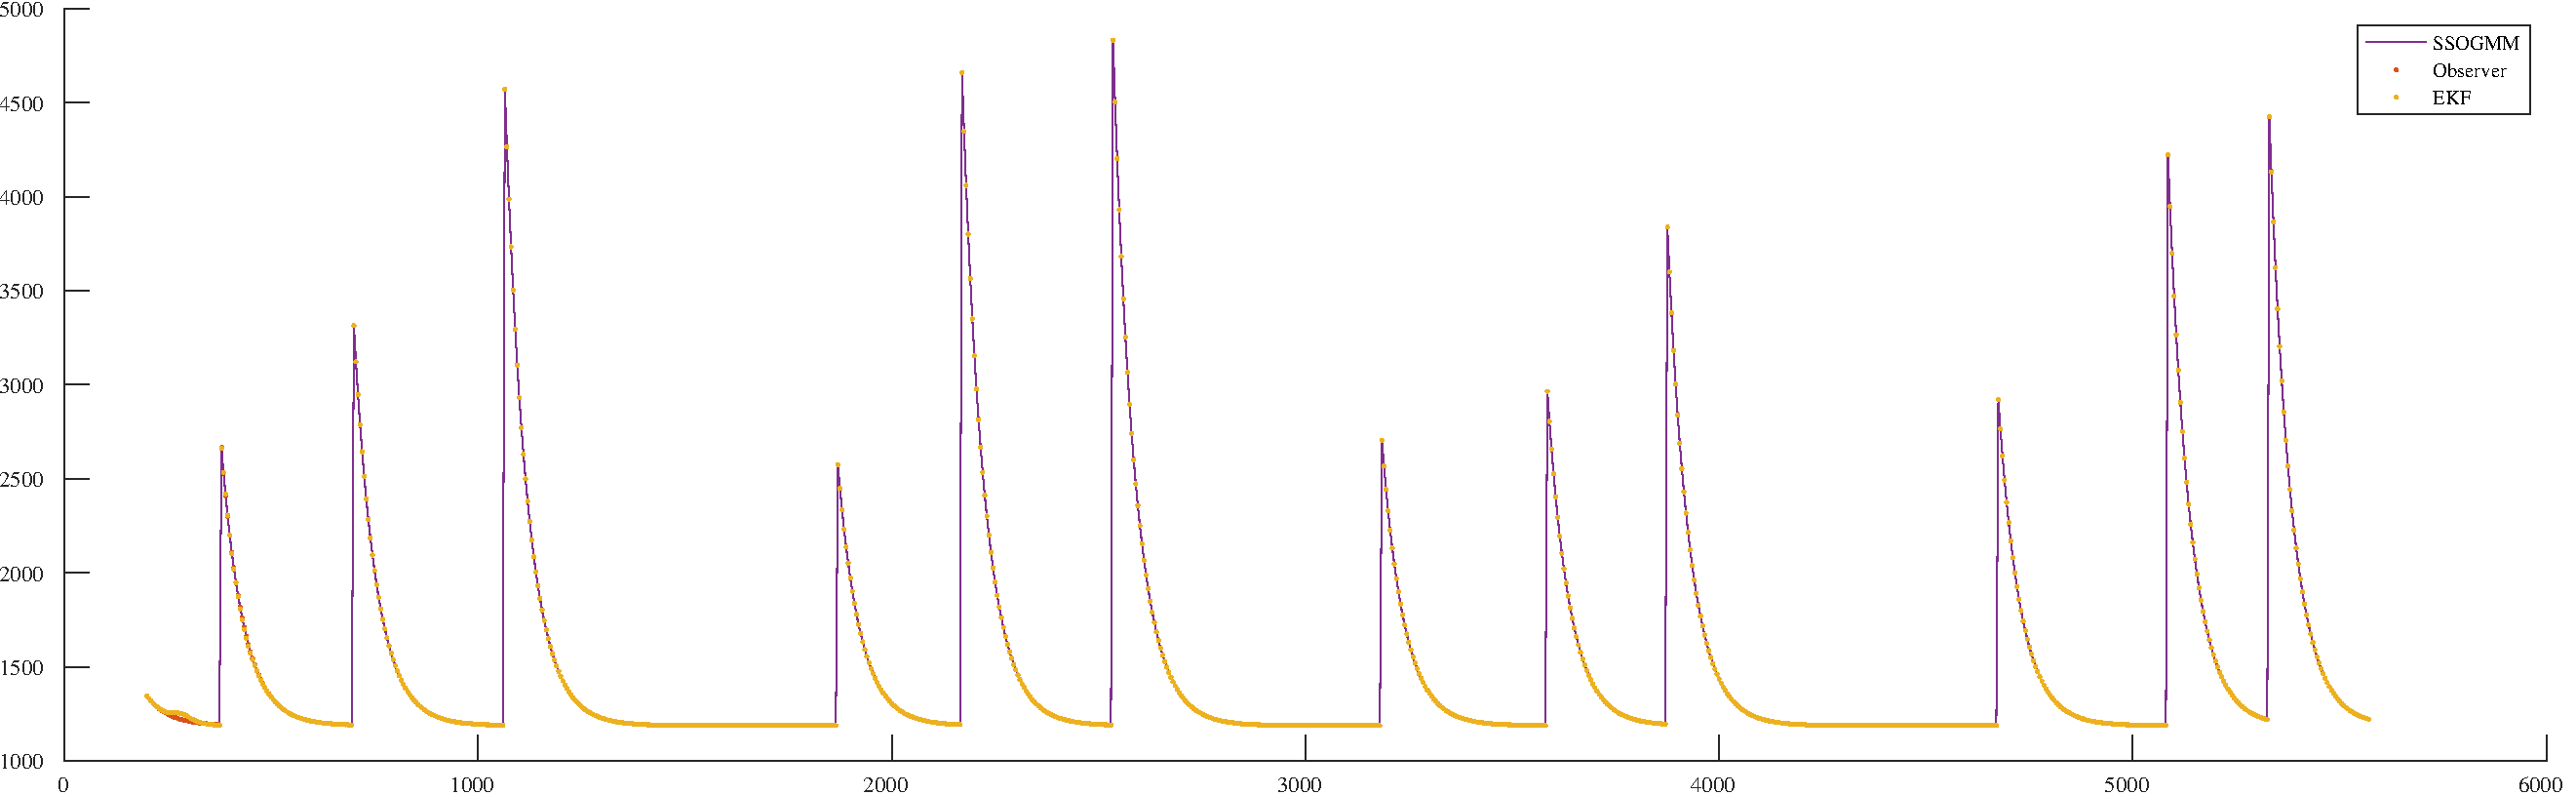
\includegraphics[width=\columnwidth]{fig/002i1.pdf}
     \caption{I1}
     \label{fig:002i1}
  \end{minipage}
%
  \begin{minipage}{0.65\columnwidth}
     \centering
     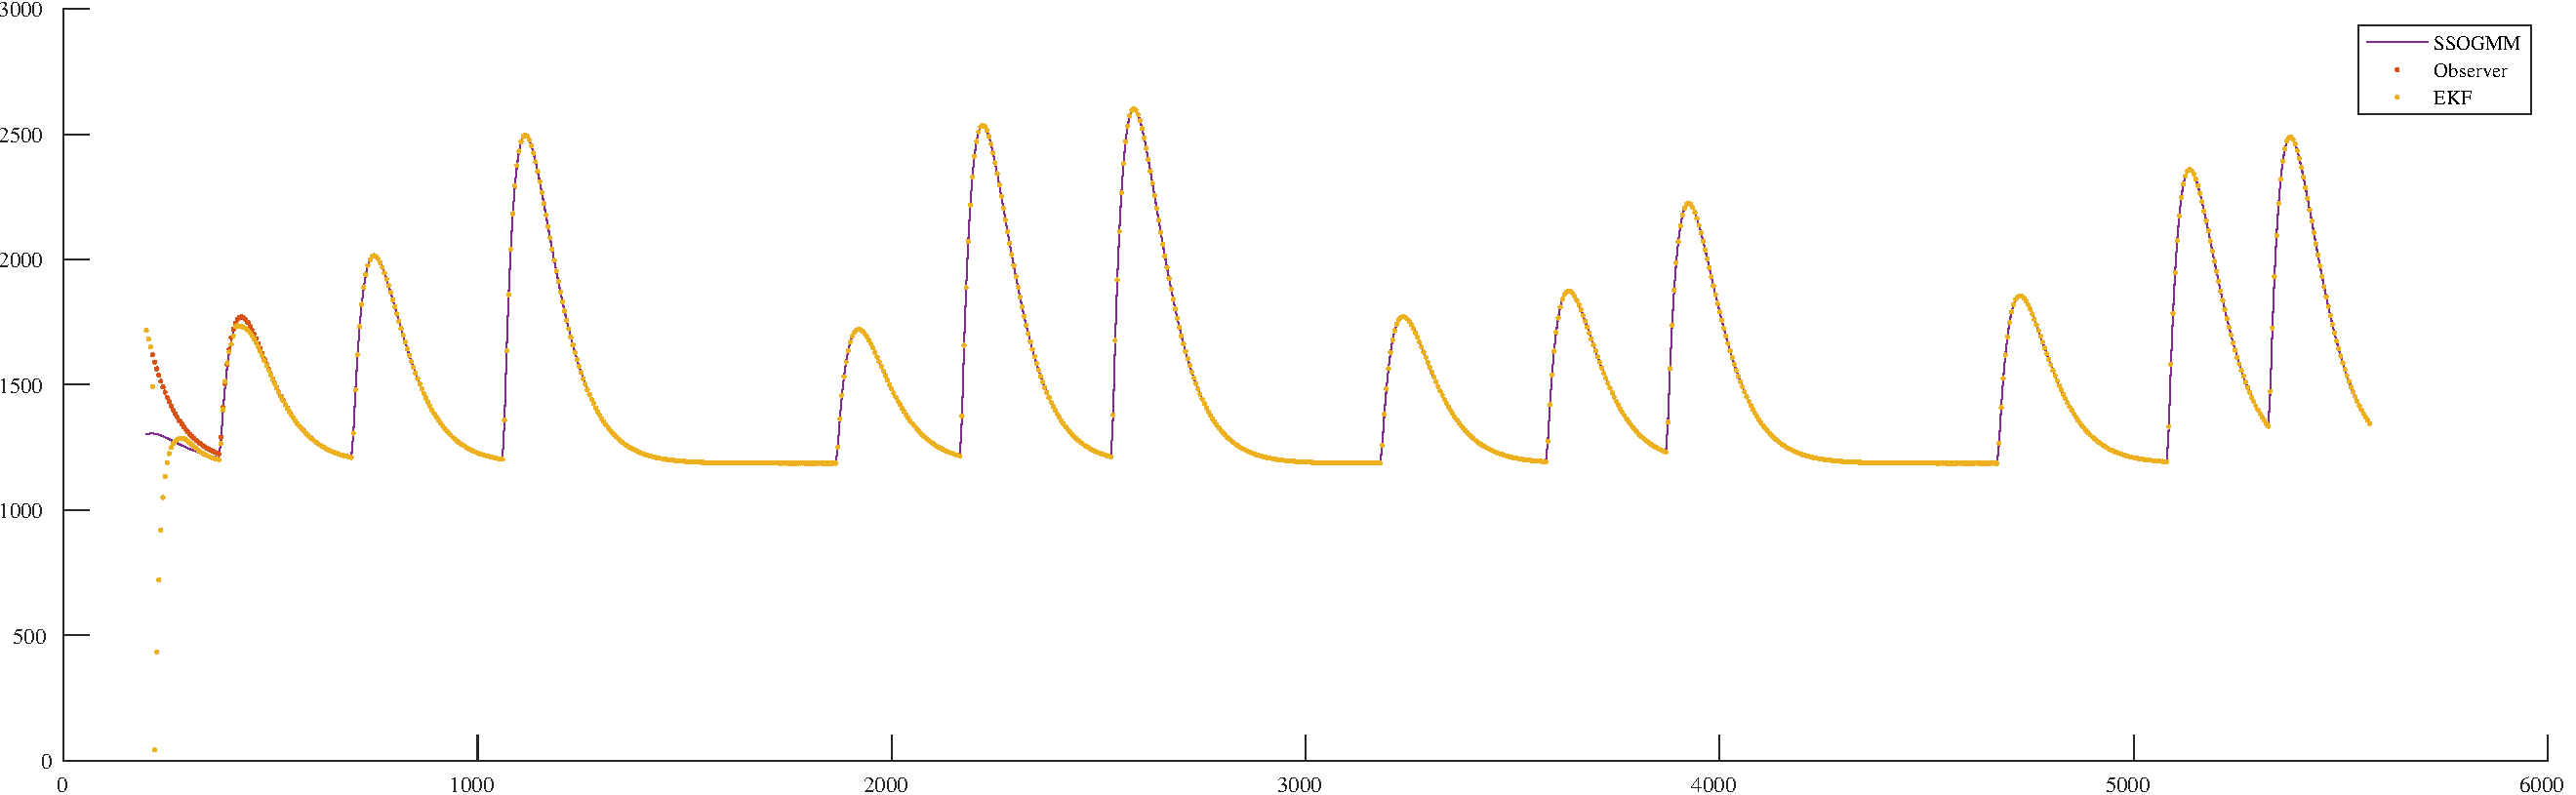
\includegraphics[width=\columnwidth]{fig/002i2.pdf}
     \caption{I2}
     \label{fig:002i2}
  \end{minipage}
%
  \begin{minipage}{0.65\columnwidth}
     \centering
     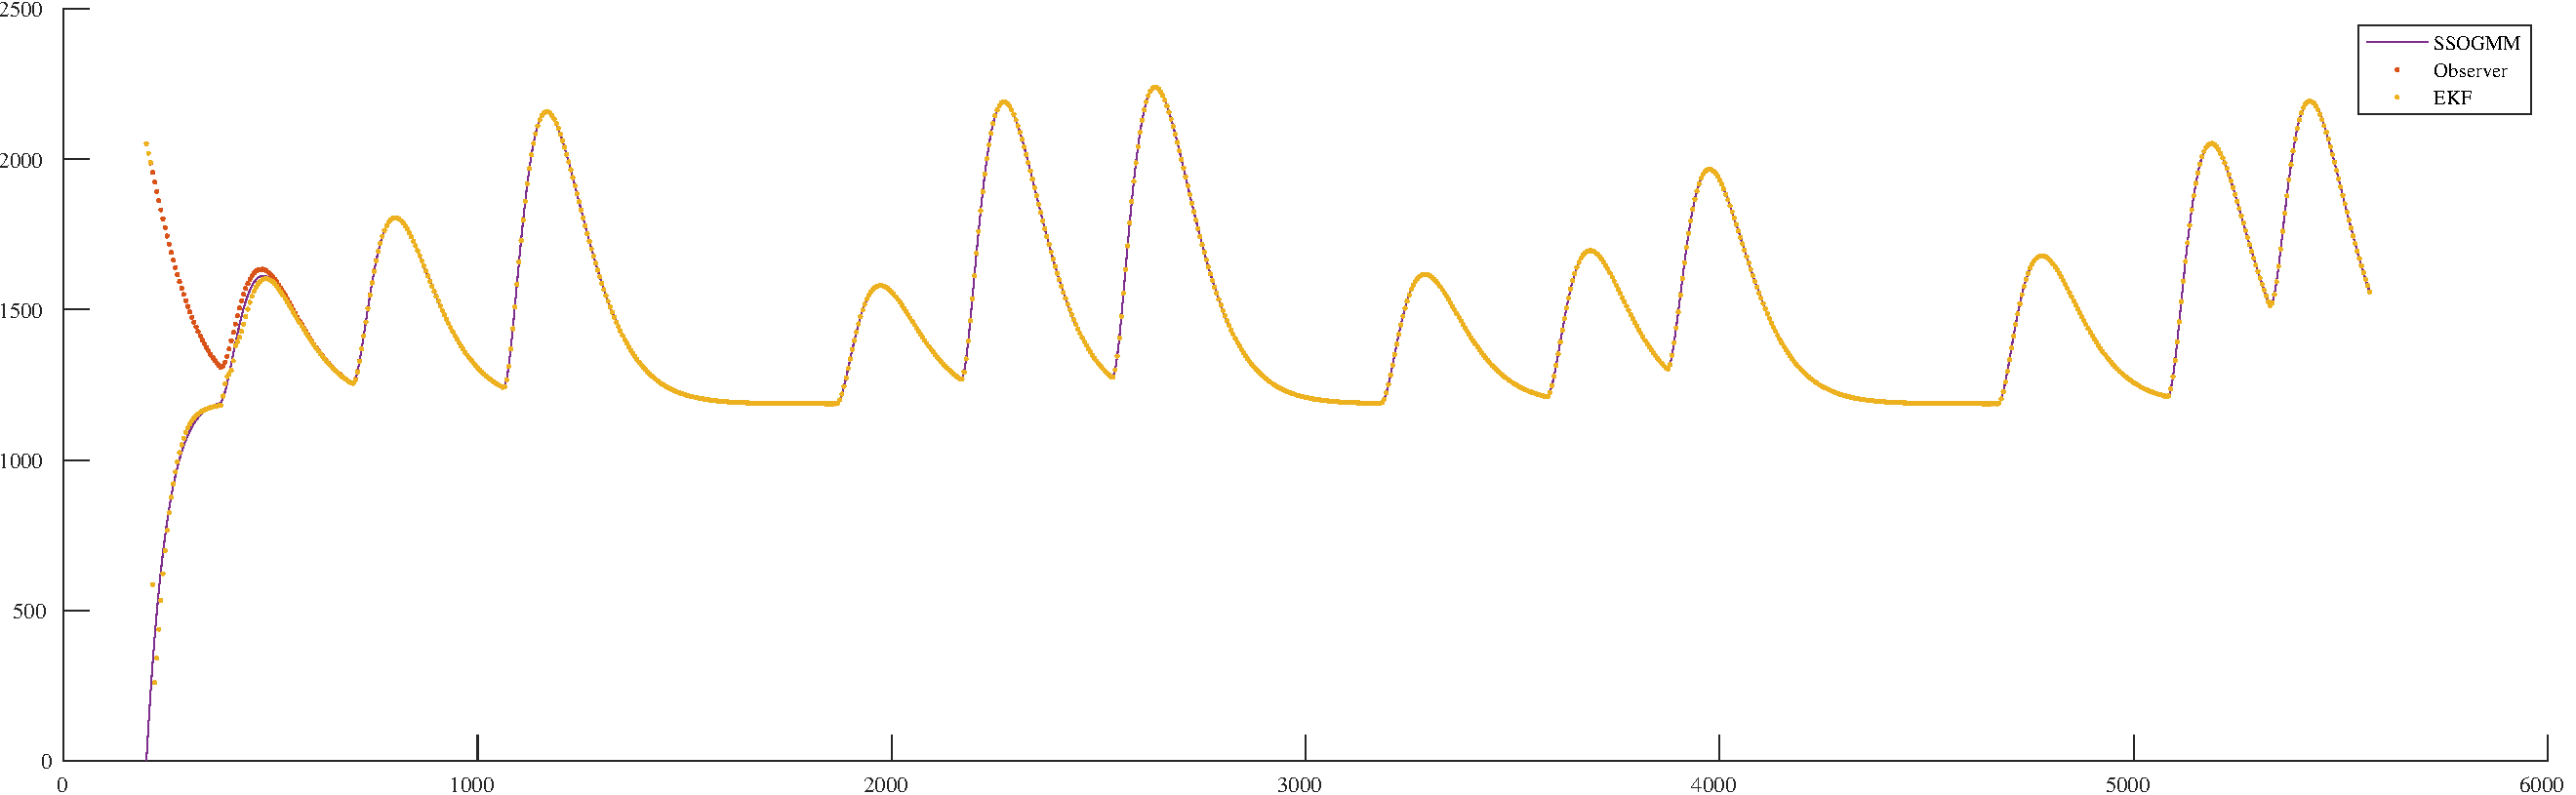
\includegraphics[width=\columnwidth]{fig/002ip.pdf}
     \caption{Ip}
     \label{fig:002ip}
  \end{minipage}
\end{figure}



\section{今後の方針}
三輪さんから過去に作ったmpcのコードの場所を教えていただいたので、そちらのコードを参考に現在の環境に合わせて、つまりSSOGMMをmpcの予測モデルとして利用できるようにコードを書き換え、とりあえず動作するとこまでの準備はできている。最終的にはUva/Padova T1DMシミュレータにmpcを実装し、シミュレーションを行っていきたいが、モードをどう与えたらいいかなど、手間取ることが多そう。なので、最初はmatlab上に実装してあるUva/Padovaモデルを使ってmcpのシミュレーションを行おうと思う。

また状態推定についても、今までモードについてはすべてわかっているとして考えてきたが、実際にはこのモードについても推定する必要があるためこの方法についても、今後考えていく必要がある。

\textcolor{red}{mpcに関するブロック線図を書く}
%%%%\section{まとめ}

\end{document}  





